\documentclass{article}

% ----------------------------------------------------------------
% Packages
\usepackage{lipsum}
\usepackage[style=ieee, defernumbers, backend=biber]{biblatex}
\usepackage[T1]{fontenc}
\usepackage[utf8]{inputenc}
\usepackage{csquotes}
\usepackage{graphicx}
\usepackage{amsmath}
\usepackage{caption}                    % for captions
\usepackage[ngerman]{babel}             % german language support
\usepackage[T1]{fontenc}                % fix non asci letter encoding
\usepackage[nottoc,numbib]{tocbibind}   % for numbering list of figures
                                        % and images and equations
% \usepackage[titles]{tocloft}            % for custom list of equations
% ----------------------------------------------------------------

% ----------------------------------------------------------------
% Setup bibliography references style
\addbibresource{literatur.bib}
% ----------------------------------------------------------------

% ----------------------------------------------------------------
% Make my custom list of equations
% TODO!!!
% ----------------------------------------------------------------

% ----------------------------------------------------------------
% Add numbering to list of figures, list of tables
\renewcommand{\listoffigures}{%
    \begingroup
    \let\section\subsection % change section to be subsection
    \tocsection
    \tocfile{\listfigurename}{lof}
    \endgroup
}
\renewcommand{\listoftables}{%
    \begingroup
    \let\section\subsection % change section to be subsection
    \tocsection
    \tocfile{\listtablename}{lot}
    \endgroup
}
% ----------------------------------------------------------------

% ----------------------------------------------------------------
% Title, author and date
\title{
    \LARGE \textbf{Laborübung II}
    \vspace{0.5cm}
    \hrule height 2pt
    \vspace{0.5cm}
    \textbf{Laborprotokoll Drehpendel}
    \vspace{0.5cm}
    \hrule height 2pt
    \vspace*{15\baselineskip}
    {
        \small Gruppenmitglieder: Lucas Hörl und Rafał Dąbek
        \\
		Betreuer: Prof. Johann Laimer
    }

}
\author{
    \textbf{Rafał Dąbek}
}
\date{
    fertiggestellt am \today \\
    \textit{Versuchsdurchführung am 29. November 2023}
}
% ----------------------------------------------------------------

% ----------------------------------------------------------------
% Make links in the document
\usepackage{hyperref}                   % for links
% Setup links
\hypersetup{
    colorlinks,
    citecolor=black,
    filecolor=black,
    linkcolor=black,
    urlcolor=black
}
% ----------------------------------------------------------------

\begin{document}

% First page with title, author and date
\maketitle
\clearpage

% Second page with table of contents
\tableofcontents
\clearpage

\section{Einleitung}
Dieses Laborprotokoll befasst sich mit der Ausmessung charakteristischer Größen eines Drehpendels nach Pohl. Das Pohlsche Rad
ermöglicht die Bestimmung der Eigenschaften des Systems bei verschiedenen Dämpfungen und Erregerfrequenzen.
Die Versuche umfassen die Bestimmung der Eigenfrequenz des Systems, die Messung an freien und erzwungenen Schwingungen bei verschiedenen Dämpfungen,
sowie auch die Bestimmung einer Resonanzkurve.

\section{Theoretische Grundlagen des Pendels}
\subsection{Differentialgleichung}
Die mathematische Beschreibung des Pendels erfolgt über eine Gleichung der Drehmomente, welche durch die folgende
Differentialgleichung 2. Ordnung beschrieben werden kann:
\begin{gather} \label{eq:pendel}
    J \cdot \ddot \varphi(t) + r \cdot \dot \varphi(t) + D \cdot \varphi(t) = M_{0} \cdot cos(\omega_{E} \cdot t)
\end{gather}
Die einzelnen Terme stehen für:
\begin{flushleft}
\begin{tabular}{lc@{ }l}
    $\varphi(t)$ & ... & die Auslenkung (Winkel) des Pendels\\
    $\dot \varphi(t)$ & ... & die Winkelgeschwindigkeit des Pendels\\
    $\ddot \varphi(t)$ & ... & die Winkelbeschleunigung des Pendels\\
    $J$ & ... & das Trägheitsmoment des Pendelkörpers\\
    $r$ & ... & der Dämpfungskoeffizient (Wirbelstrombremse)\\
    $D$ & ... & die Winkelrichtgröße\\
    $M_{0}$ & ... & die Amplitude des Drehmoments des Erregers\\
    $\omega_{E}$ & ... & die Erregerfrequenz
\end{tabular}
\end{flushleft}
Das Trägheitsmoment wird definiert als $J = \rho \cdot \int_{V}^{} r^{2} dV$.
\cite{w:traegheit}

\subsection{Die Lösung der Differentialgleichung}
\subsubsection{Freie Schwingung}
Die freie Schwingung findet statt, wenn der Dämpfungsterm und Erregerterm wegfallen, d.h. $r = 0$ und $M_{0} = 0$.
Die Differentialgleichung lautet dann:
\begin{gather} \label{eq:freie_schwingung}
    J \cdot \ddot \varphi(t) + D \cdot \varphi(t) = 0\\
    \ddot \varphi(t) + \frac{D}{J} \cdot \varphi(t) = 0
\end{gather}
Die Lösung erfolgt durch den Exponentialansatz:
\begin{gather} \label{eq:freie_schwingung_ansatz}
    \varphi(t) = A \cdot e^{\lambda \cdot t}\\
    \ddot \varphi(t) = \lambda^{2} \cdot A \cdot e^{\lambda \cdot t}
\end{gather}
Dadurch entsteht die charakteristische Gleichung:
\begin{gather} \label{eq:freie_schwingung_loesung}
    \lambda^{2} + \lambda \cdot \frac{D}{J} = 0\\
    \lambda = \pm i \cdot \sqrt{\frac{D}{J}}
\end{gather}
Sehr praktisch ist hier $\omega_{0}$ zu definieren als $\omega_{0} = \sqrt{\frac{D}{J}}$, bzw. $\omega_{0}^{2} = \frac{D}{J}$.
Somit ist $\lambda = \pm i \cdot \omega_{0}$. Die Lösung ist dann
$\varphi(t) = A_{1} \cdot e^{-i \omega_{0} \cdot t} + A_{2} \cdot e^{i \omega_{0} \cdot t}$.
Durch die Eulersche Identität $e^{i \cdot \varphi} = cos(\varphi) + i \cdot sin(\varphi)$ kann auf die Form
$\varphi(t) = B_{1} \cdot cos(\omega_{0} \cdot t) + B_{2} \cdot sin(\omega_{0} \cdot t)$ umgeformt werden. Mit den Anfangsbedingungen
\begin{gather} \label{eq:freie_schwingung_loesung}
    \varphi(t = 0) = \varphi_{0}\\
    \dot \varphi(t = 0) = 0
\end{gather}
ergibt sich die Lösung:
\begin{gather} \label{eq:freie_schwingung_loesung}
    \varphi(t) = \varphi_{0} \cdot cos(\omega_{0} \cdot t)
\end{gather}
\subsubsection{Gedämpfte Schwingung}

\subsubsection{Aperiodischer Grenzfall}
\subsubsection{Kriechfall}
\subsection{Die Lösung der inhomogenen Differentialgleichung}
\subsubsection{Resonanzkurven}
\subsection{Schwebung}
\clearpage

\section{Versuchsaufbau}
Der Versuchsaufbau bestand aus einem Drehpendel nach Pohl der Firma Leybold \ref{fig:versuchsaufbau}.
Für die Messungen stand das Programm CASSY auf einem Labor-PC zur Verfügung.
Das Messystem erfasste automatisch über die entsprechende Schnittstellen \ref{fig:schnittstelle}
nach dem Start einer Aufzeichnung die Bewegung des Pendelkörpers
über den BMW (Bewegungsmesswandler). Diese Daten wurden dann in der CASSY-Software
und in Microsoft Excel ausgewertet.

\begin{figure}
    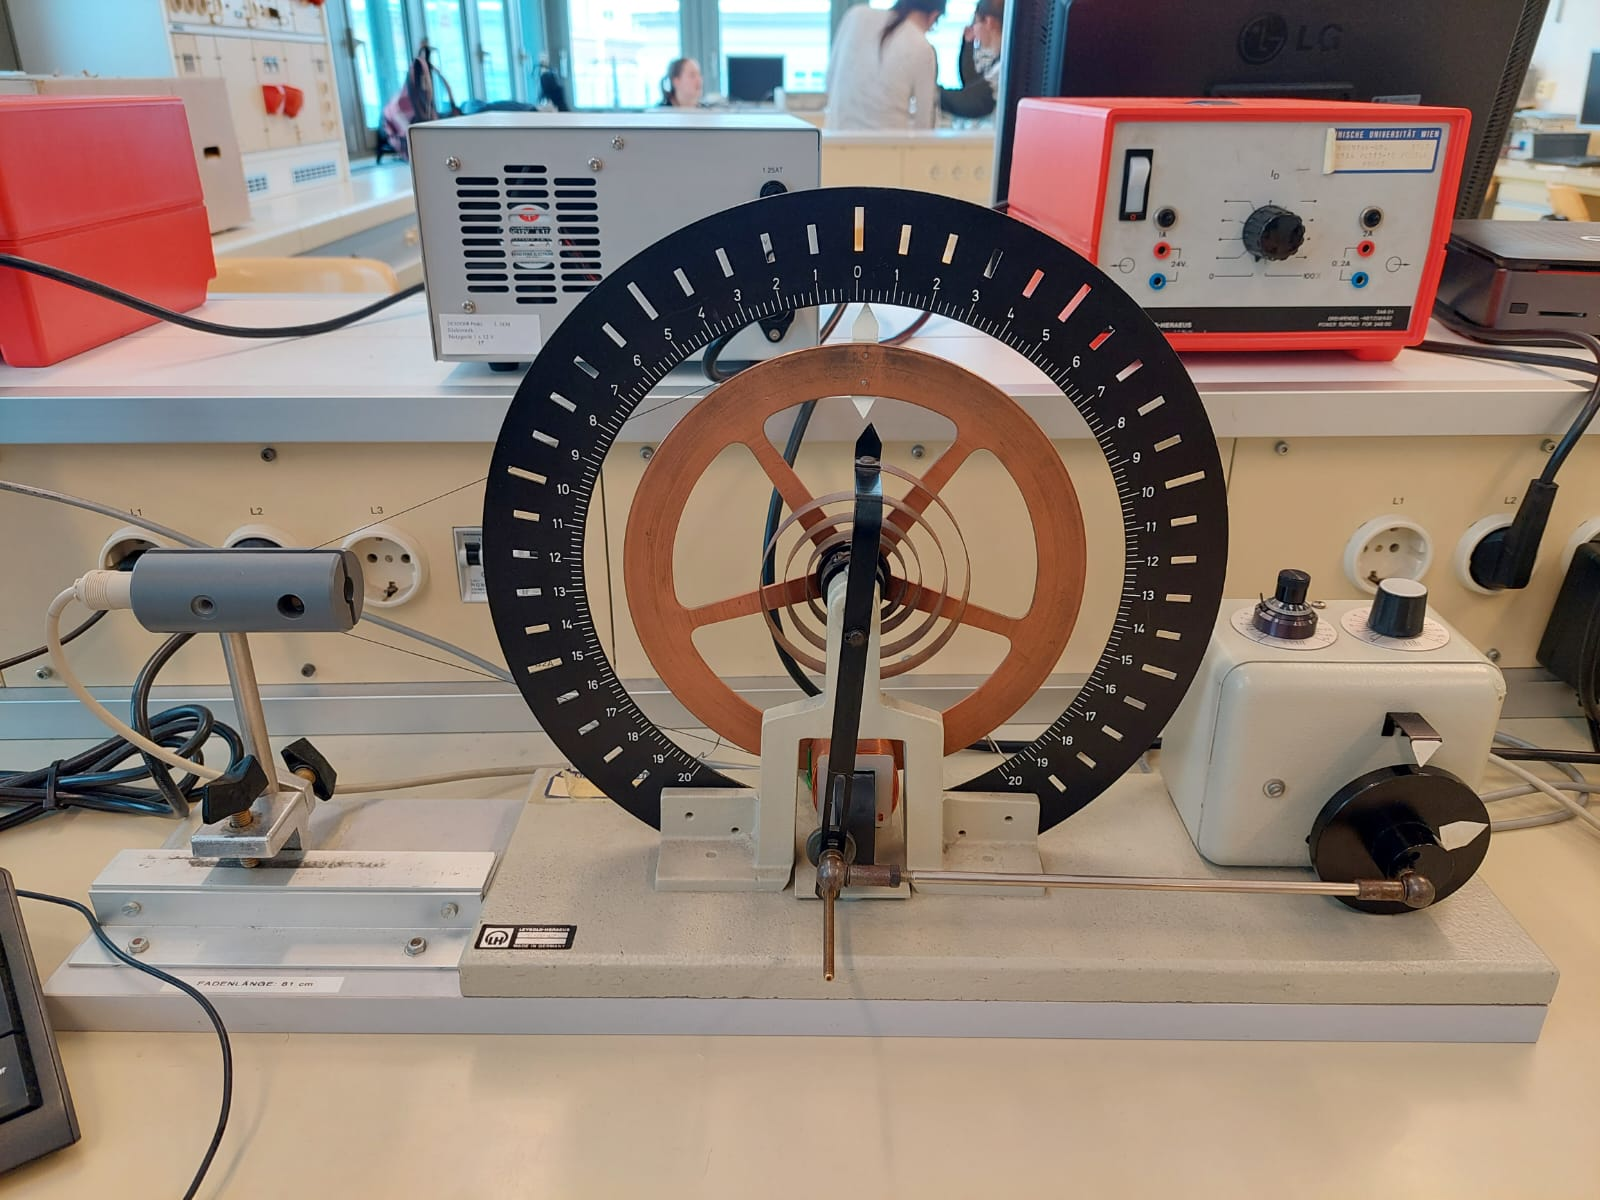
\includegraphics[width=\linewidth]{bilder/drehpendel.jpg}
    \caption{Ein Foto des Versuchsaufbaus}
    \label{fig:versuchsaufbau}
\end{figure}

\begin{figure}
    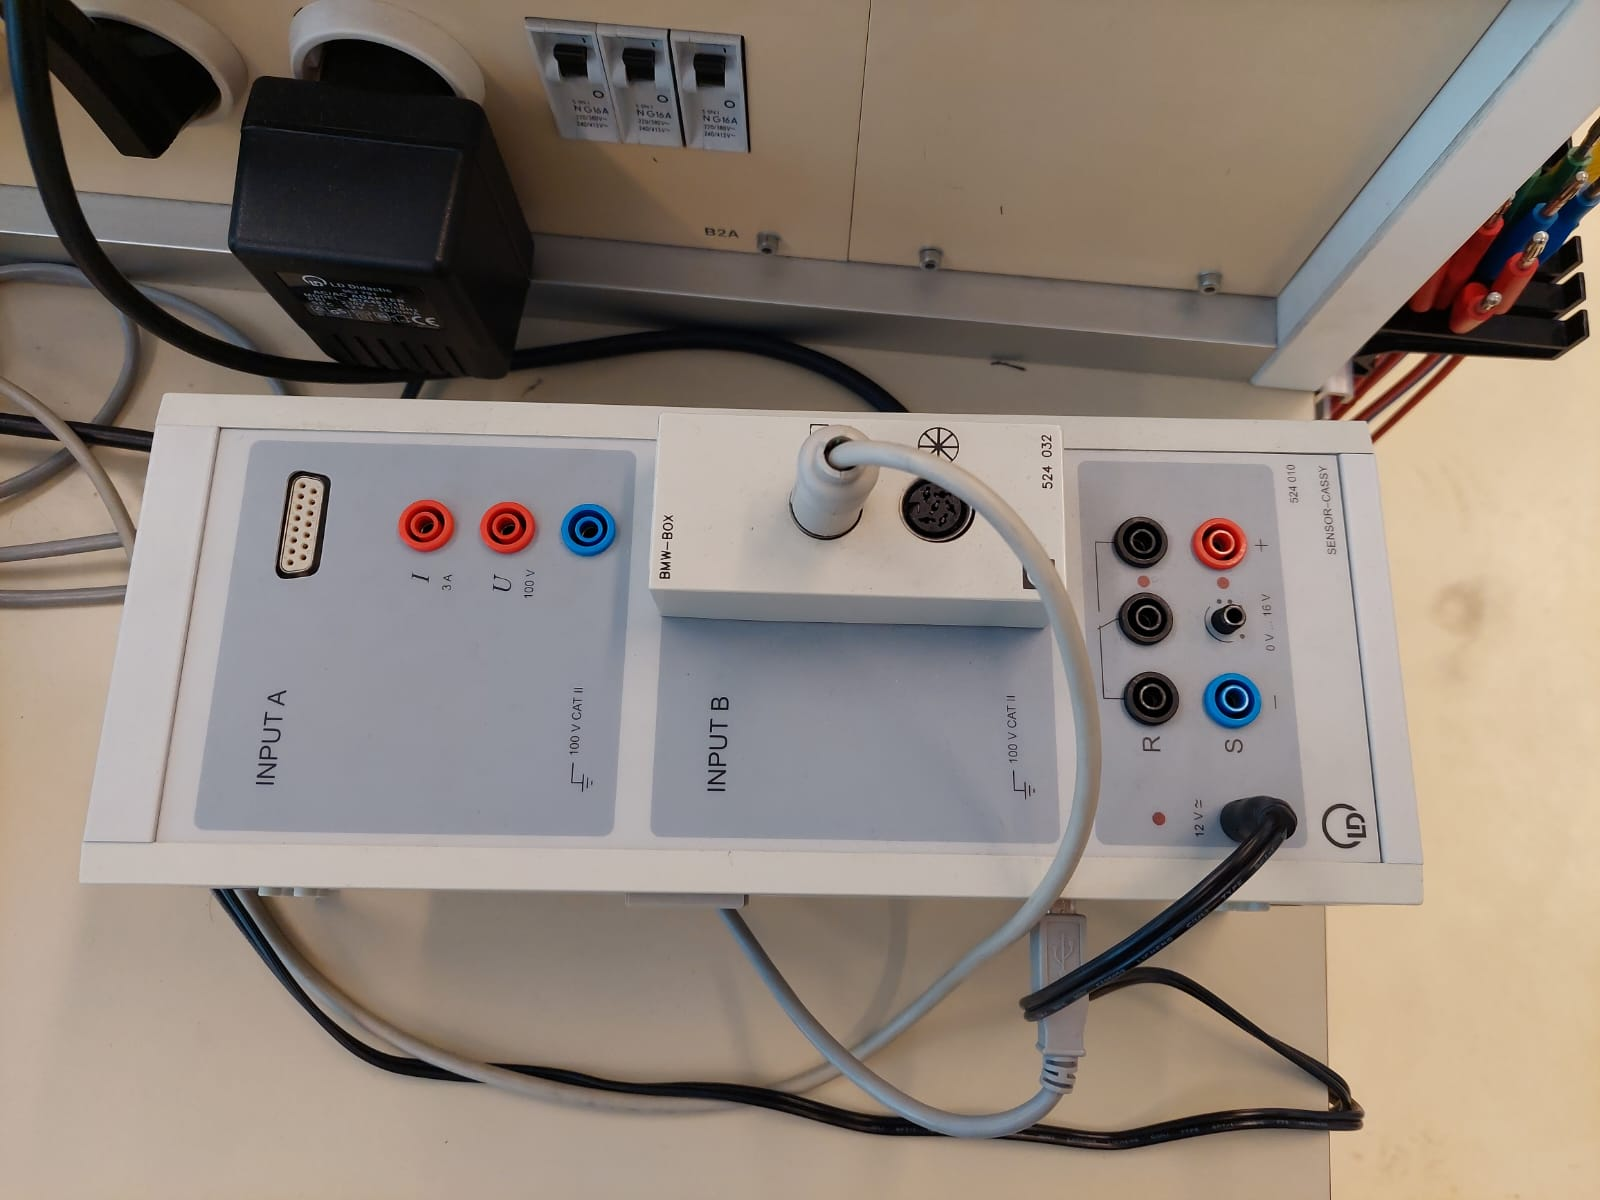
\includegraphics[width=\linewidth]{bilder/sensor_cassy.jpg}
    \caption{Ein Foto der Schnittstelle}
    \label{fig:schnittstelle}
\end{figure}

Der Aufbau des Pendels \cite{w:pohl} besteht aus einem Kupferrad, welches das Pendel simulieren soll.
Das Kupferrad ist über eine Nabe an eine Feder verbunden. Diese bewirkt das entsprechende
Rückstellmoment. Außerdem kann das Pendel über einen Hebel, der exzentrisch an einem
elektrischen Motor befestigt ist, angetrieben werden. Letzendlich kann mit einer Wirbelstrombremse
eine zusätzliche Dämpfung eingestellt werden.

\begin{figure}
    \includegraphics[width=\linewidth]{}
    \caption{Das Pendel nach Pohl}
    \label{fig:pendel}
\end{figure}
\clearpage

\section{Versuche}
\subsection{Bestimmung der Eigenfrequenz}
\subsubsection{Durchführung}
Das Ziel dieses Versuches war es die Eigenfrequenz und die Abklingkonstante zu
bestimmen. Die Dämpfung sollte dabei nicht vorhanden sein, d.h. die Wirbelstrombremse
sollte ausgeschaltet bleiben. Die Bestimmung der Eigenfrequenz erfolgte über
die Messung der Zeit $\delta t$ über mehrere Perioden n. Die Frequenz wird dann
folgendermaßen berechnet: $f = \frac{n}{\delta t}$.

Die Abklingkonstante $\delta$ konnte mittels CASSY aus dem Wert $B$ folgend
bestimmt werden: $\delta = \frac{1}{B}$, wobei $B$ aus der Messung abgelesen werden konnte.
\subsubsection{Messdaten}

\subsubsection{Auswertung}
\begin{center}
\begin{tabular}{c c c}
    \hline
    1st & 2nd & 3rd \\
    \hline
    A & B & C \\
    D & E & F \\
    \hline
\end{tabular}
\captionof{table}{\label{demo-table}Some table.}

\subsection{Schwingung bei verschiedenen Dämpfungen}
\subsubsection{Durchführung}
\subsubsection{Messdaten}
\subsubsection{Auswertung}

\subsection{Zusammenhang Erregerfrequenz und Erregerspannung}
\subsubsection{Durchführung}
\subsubsection{Messdaten}
\subsubsection{Auswertung}

\subsection{Resonanzkurve}
\subsubsection{Durchführung}
\subsubsection{Messdaten}
\subsubsection{Auswertung}

\clearpage

\section{Diskussion}
\clearpage

\section{Anhang}
\subsection{Verwendete Geräte}
\begin{itemize}
    \item Bewegungsmesswandler der Firma Leybold, Type 524 082
    \item Software Cassy Lab der Firma Leybold, Type 524 220
    \item Drehpendel nach Pohl der Firma Leybold, Type 34600-B2
\end{itemize}
\listoffigures
\listoftables
\printbibheading[title={Literaturverzeichnis},heading=subbibnumbered]
% \printbibliography[type=book,heading=subbibliography,title={\indent \textit{Bücher}}]
\printbibliography[type=online,heading=subbibliography,title={\indent \textit{Webseiten}}]

\end{document}